\chapter{Theoretical Background and Related Work}
\label{chapter:background} 

In chapter \ref{chapter:intro} a brief general analysis of stereo geometry and methods has been provided. 
In this chapter a more precise revision of the theoretical tools that stereo matching methods exploit is presented.
Epipolar geometry, camera calibration and disparity estimation algorithms are specifically described. 
Starting from the necessary mathematical basis, the discussion moves on the disparity estimation algorithms. 
Then, the chapter focus on the main benefits and drawbacks of standard and novel approaches in depths computation.
Comparison between stereo-geometry based and deep learning based algorithms is proposed, to provide a clear explanation of the decisions implemented. 

\section{Epipolar geometry and Rectifiation}
\label{sec:eipolarandrect}

Fundamental problem of stereo vision is the estimation of 3D locations of points from at least two corresponding input images.
This process, which comprises concurrent computation of both 3D geometry and camera pose, is generally known as structure from motion \cite{Szeliski2011}.\\
In the explanation of these topics it is necessary to start discussing about the triangulation.
Then, the concept of epipolar geometry is outlined and after that the notions of camera calibration and rectification. 

\subsection{Triangulation}
\label{subsec:triangulation}

\begin{figure}[t]
	\begin{center}
		{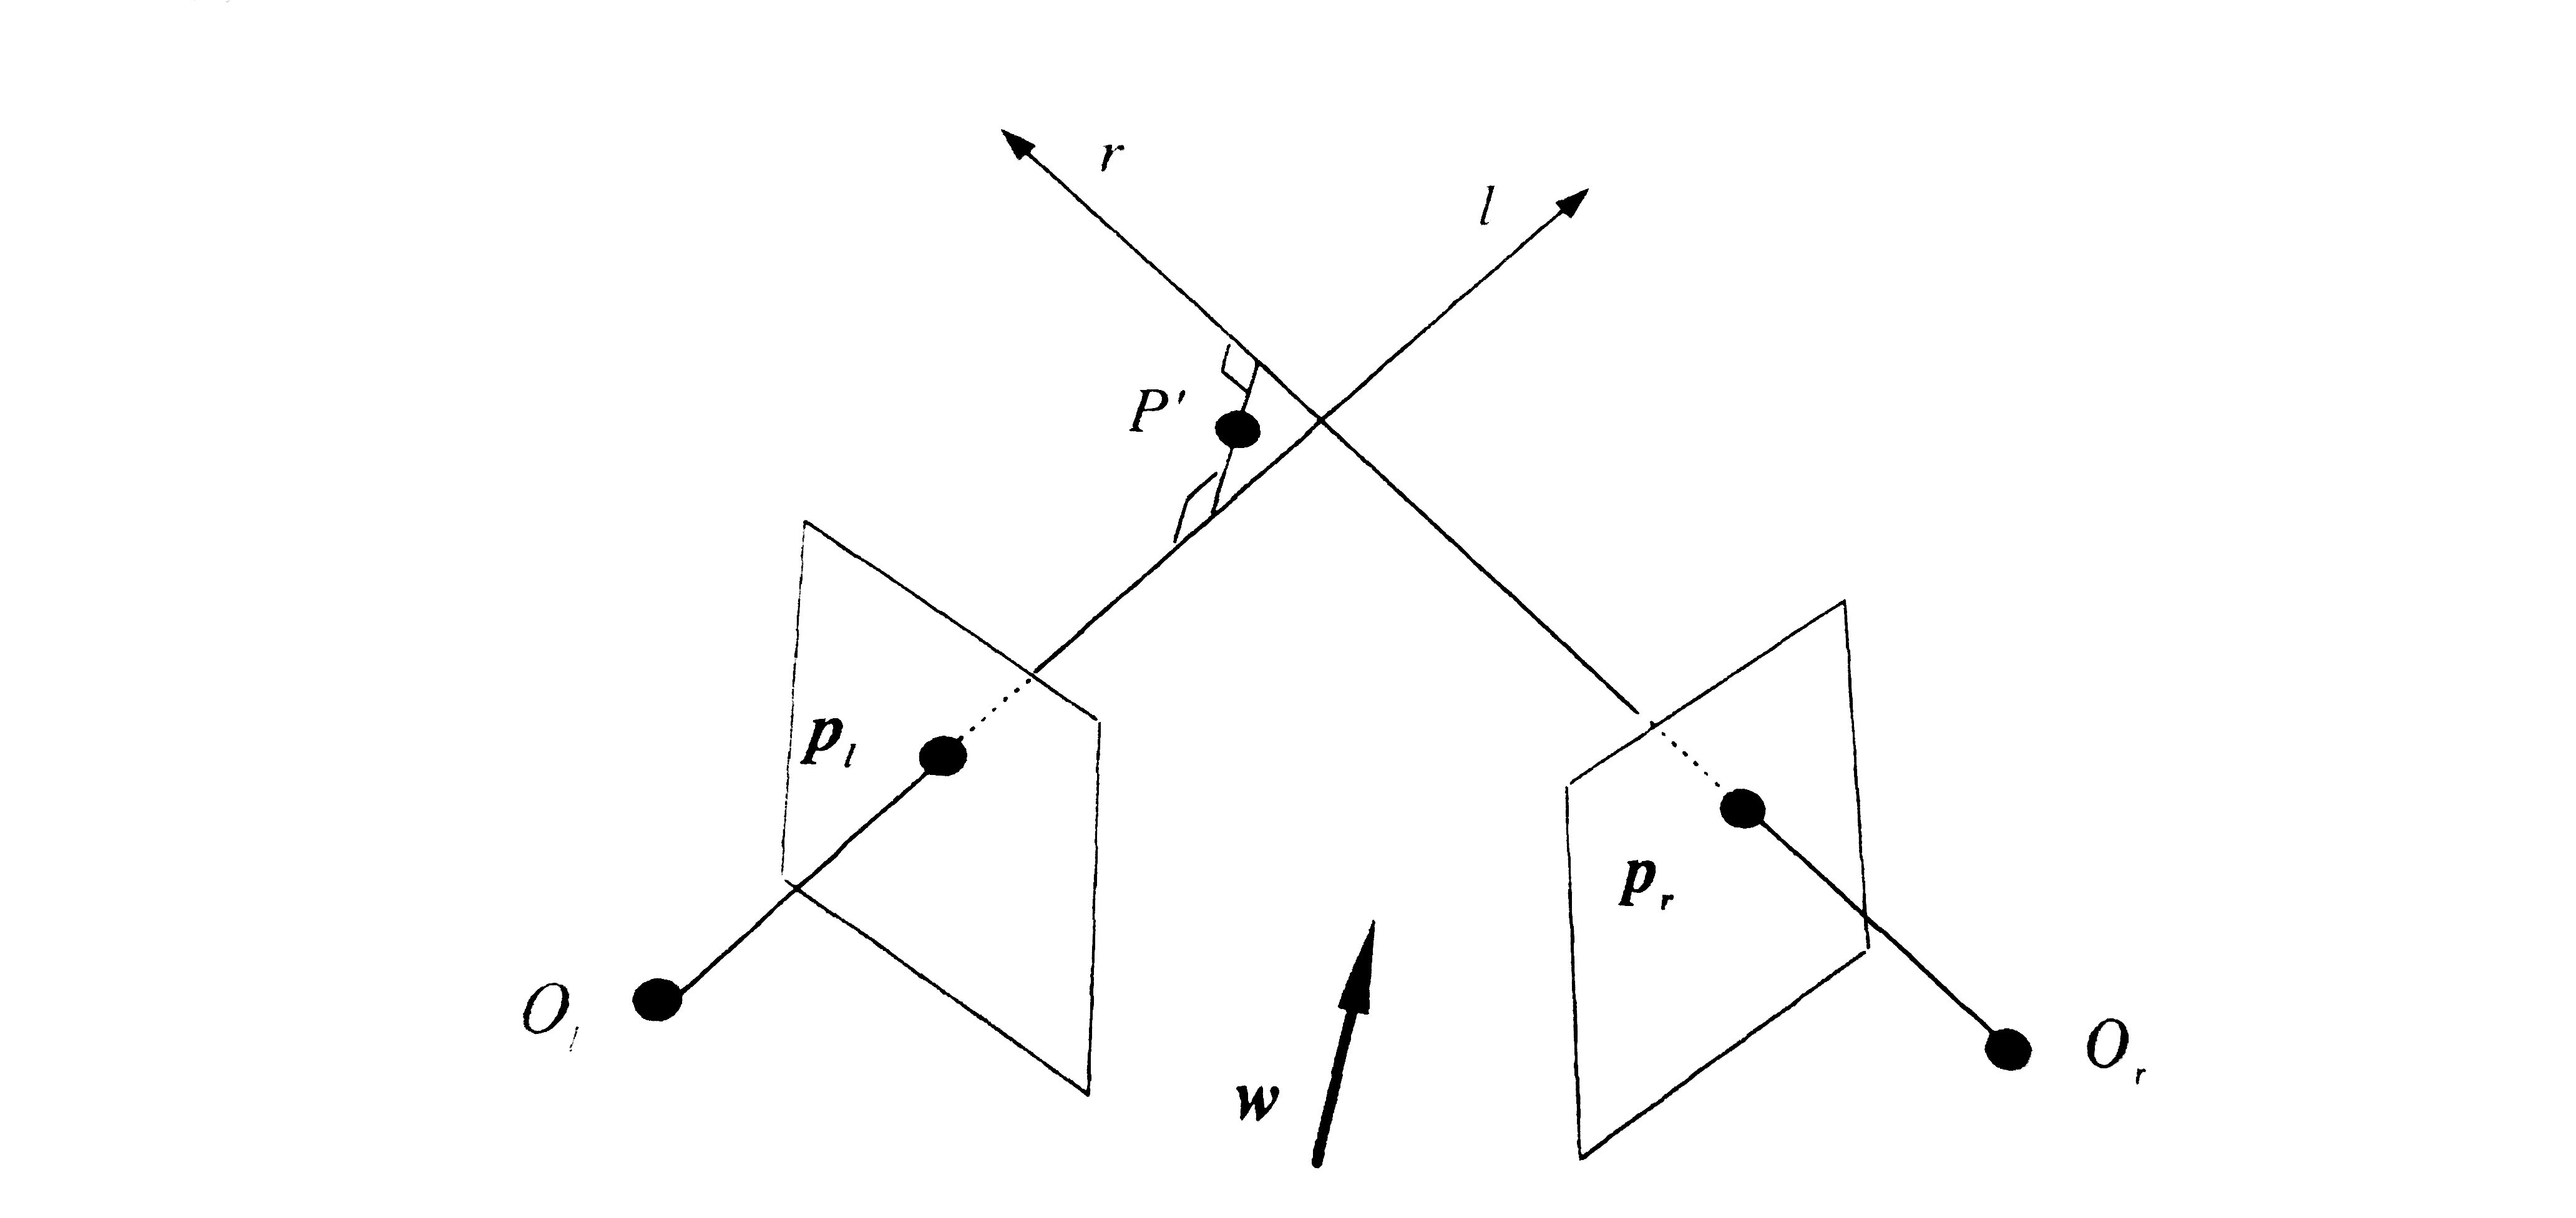
\includegraphics[width=.8\textwidth]{images/triangulation}}
\caption{3D triangulation by finding point $P'$ that lies nearest to all of the optical rays}
\label{fig:triangulation}
	\end{center}
\end{figure}

Triangulation is the problem of detecting 3D points positions from a collection of corresponding 2D image locations, assuming that camera positions are known.
Figure \ref{fig:triangulation} shows one of the easiest methods to tackle this problem. 
Objective is to evaluate the 3D position of $P'$ that have the smallest error to all of the 3D optical rays coming from the camera centers, which identify the 2D point locations in the image plane, i.e. $P_r$ and $P_l$.
As shown in Figure \ref{fig:triangulation}, the rays starts from the camera centers, $O_j$ and go in direction of $r$ and $l$, which can be defined using the camera matrix $ \{ P_j = K_j [ R_j | t_j ] \} $.
The closest point to $P$ on this ray minimizes the distance
\begin{equation}\label{eqn:mindist}
	\Vert O_j + d_j \hat{v}_j - P \Vert^2
\end{equation}
Therefore, because of the minimum is $d_j = \hat{v}_j \cdot (p - c_j)$, the nearest points are calculated as:
\begin{equation}\label{eqn:closestpoint}
	q_j = O_j + (\hat{v}_j \hat{v}_j^\top)(P - O_j) = O_j + (P - O_j)_{\Vert}
\end{equation}
Hence, the optimal value for $P$, obtained solving a least square problem, becomes,
\begin{equation}\label{eqn:solP}
	P = \Big[ \sum_j (I - \hat{v}_j \hat{v}_j^\top ) \Big]^{-1} = \Big[ \sum_j (I - \hat{v}_j \hat{v}_j^\top )O_j \Big]
\end{equation}

\subsection{Epipolar geometry}
\label{subsec:epipolargeom}

\begin{figure}[t]
	\begin{center}
		{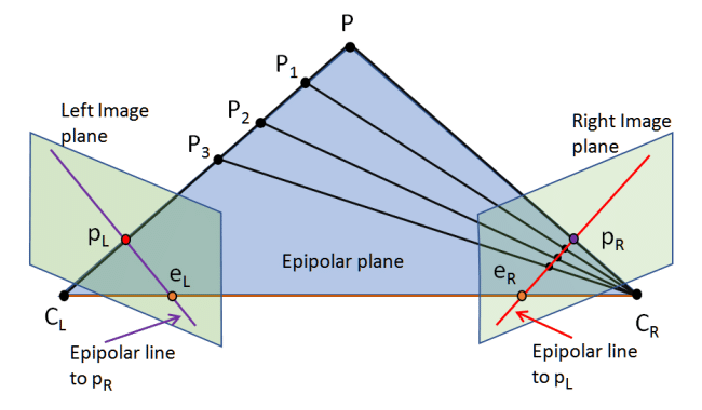
\includegraphics[width=.8\textwidth]{images/epipolar-geometry-2}}
\caption{Epipolar geometry. Image point $m$ back-projects to a ray in a 3D space defined by $C$ and $m$. This ray becomes a line $l'$ in the second view. The image of $X$ must lie on $l'$}
\label{fig:epipolargeom-2}
	\end{center}
\end{figure}

The intrinsic projective geometry between two views is known as epipolar geometry.
It is only dependent on the cameras' internal parameters and pose.
The $3 \times 3$ rank 2 matrix that defines this geometry is the fundamental matrix $F$.\\
The epipolar geometry is the basis for finding corresponding points in stereo matching. 
It is basically defined by the intersection between image planes and the one on which the cameras baseline lies.\\
A fundamental property, that makes this geometry extremely useful, is that image points, space point and camera centers are coplanar. 
Assuming that only $m_l$ is known, that geometry allows to constraint the corresponding point $m_r$. 
The epipolar plane is defined by the baseline and the ray that comes from $m_l$. 
Hence, knowing that $m_r$ lies on the same plane, that point belongs to $l_r$, i.e. the intersection between the epipolar and the second image plane. 
Therefore, exploiting this property, the searching of corresponding points is constrained to only one line inside the image. 


\section{Stereo methods and dense correspondence}
\label{sec:stereometh}
Never ever copy anything into your theses from somebody else's text
(nor your own previously published text). Never. Not even for starting
point to be rewritten later. The risk is that you forgot the copied
text to your thesis and end up to be accused of plagiarism. Plagiarism
is a serious crime in studies and science and can ruin your career
even its beginning. To repeate: never cut and paste text into your
thesis!

\subsection{Stereo geometry based methods}

\subsection{Deep learning based methods}

All work is based on someone else's work. You should find the relevant
sources of your field and choose the best of them. Also, you should
refer to the original source where a fact has been mentioned first
time. Remember source evaluation (criticism) with all sources you
find.

Good starting points for finding references in computer science are: 
\begin{itemize}
% You can use this command to set the items in the list closer to each other
% (ITEM SEParation, the vertical space between the list items) 
\setlength{\itemsep}{0pt}
\item Aalto library's Computer Science Guide: \url{http://libguides.aalto.fi/computer} 
(in English) and \url{http://libguides.aalto.fi/tietotekniikka} (in Finnish)
\item Finna Portal (Aalto Library): \url{https://aalto.finna.fi/?lng=en-gb} (in English) 
and \url{https://aalto.finna.fi/} (in Finnish)
\item ACM Digital library: \url{http://portal.acm.org/}
\item IEEExplore: \url{http://ieeexplore.ieee.org}
\item ScienceDirect: \url{http://www.sciencedirect.com/}
\item \ldots although Google Scholar (\url{http://scholar.google.com/}) will
find links to most of the articles from the abovementioned sources, if you
search from within the university network
\end{itemize}

Some of the publishers do not offer all the text of the articles
freely, but the library has agreed on the rights to use the whole
text. Thus, you should sometimes use computers in the domain of the
university in order to get the full text. Sometimes the Finna Portal
can also help getting the whole article instead of just the abstract.
The library has also a self-study guide to information retrieval~\cite{howfindinfo}.

Instead of normal Google, use Google Scholar
(\url{http://scholar.google.fi/}). It finds academic publications whereas
normal Google find too much commercial advertisements or otherwise
biased information. Wikipedia articles should be referred to in the master
thesis only very, very seldomly. You can use Wikipedia for understanding
some basics and finding more sources, but often you cannot be sure if
the article is correct and unbiased.

One important part of the sources that you have found is the reference
list. This way you can find the original sources that all the other
research of the field refer. Often you can also find more information
with the name of the researchers that are often referred in the
articles.

\subsection{Sources and reference list}

The main point in referring to sources is to separate your own
thinking and text from that of others. Facts of the research area can
be given without reference, but otherwise you should refer to
sources. This means two things: marking the source in the text where
it has been used, and listing the sources usually in the end of the
thesis in a way that help the reader to find the original source. 
Aalto library has a comprehensive citation guide
~\cite{bibinstructions}.

There are several bibliography styles, meaning how to form the
bibliography in the end of the thesis and how to mark the references
in the text. You should ask from your supervisor or instructors which
style you should use. This thesis template uses the number style that
is often used in software engineering. Here, the bibliography is in
the alphabetical order, not in the order where the sources are
referred, and the sources are marked with numbers in the text. In all
styles, the key idea is to collect as much information of the sources
as is possible in the bibliography, and then let the latex environment take
care of organizing the necessary information to the reference list.

The other bibliographic styles are also used in the CS field. For example, usability
uses the Harvard style where instead of numbers, the reference is
marked into the text with author's name and publishing year. You can
change the bibliography style in the thesis-example.tex file. You get
the normal text reference, e.g. (Haapasalo, 2010), with latex command
\texttt{citet} or the plain \texttt{cite}, and with command
\texttt{citep}, you get the text reference ``Haapasalo (2010)'' that
you can use as subject of a sentence. Next, we tell more about how to mark
the references in the text.

\subsection{Referring to sources}

In addition to the list in the end of the thesis, you have to mark the
source in the text where the source is used. There are three places
for the reference: in a sentence before the period, in the end of a
sentence after the period, or in the end of a paragraph. All of them
have different meaning. The main point is that first you paraphrase
the source using your own words and then mark the source. Next, we
give short examples that are marked with \emph{emphasised text}.

\emph{Haapasalo~\cite{HaapasaloThesis} researched database algorithms
  that allows use of previous versions of the content stored in the
  database.} This kind of marking means that this paragraph (or until
the next reference is given) is based on the source mentioned in the
beginning.  Giving the source you should use only the family name of
the first author of the article, and not give any hints about what is
the type of the article that is referred nor its title.

\emph{B+-trees offers one way to index data that is stored in to a
  database. Multiversion B+-trees (MVBT) offer also a way to restore
  the data from previous versions of the database. Concurrent MVBT
  allows many simultaneous updates to the database that is was not
  possible with MVBT.~\cite{HaapasaloThesis}} When the marking is
after the period, the reference is retrospective: all the paragraph
(or after previous reference marking) is based on the source given in
its end. If the content is very broad, you can start with saying
\emph{According to Haapasalo}, then continue referring the source with
several separate sentences, and in the end put the marking of your
source \emph{ that shows that CMVBT are the
  best. ~\cite{HaapasaloThesis}}. 

If your paragraph has several sources, the above mentioned styles are
not proper. The reader of your thesis cannot know which of your
sources give which of the statements. In this case, it is better to
use more finegraded refering where the reference markings that are
embedded in the sentences. For example, \emph{the multiversion B+-tree
  (MVBT) index of Becker et al.~\cite{becker:1996:mvbt} allows database
  users to query old versions of the database, but the index is not
  transactional.
  It's successor, the transactional MBVT (TMVBT), allows a single transaction
  running in its own thread or process to update the database concurrently
  with other transactions that only read the
  database~\cite{haapasalo:2009:tmvbt}. 
  Further development, titled the concurrent MBVT (CMVBT),
  allows several transactions to perform updates to the database at the same
  time~\cite{HaapasaloThesis}}. 
  Here, the references are marked before
  the period in the sentences where they are used. You should never
  but all these sources in the end of the paragraph. Referring several
  source at once should only used when you give a set of examples.

Finally, direct quotes are allowed. However, often you should avoid
them since they do not usually fit in to your text very well. Using
direct quotes has two tricks: quotation marks and the source.  \emph{
  ``Even though deletions in a multiversion index must not physically
  delete the history of the data items, queries and range scans can
  become more efficient, if the leaf pages of the index structure are
  merged to retain optimality.''~\cite{HaapasaloThesis}} Quotes are
hard to make neatly since you should use only as much as needed
without changing the text. Moreover, you often do not really
understand what the author has mentioned with his wordings if you
cannot write the same with your own words. Remember also that never
cut and paste anything without marking the quotation marks right away,
and in general, never cut and paste anything at all!

Sometimes getting the original source can be almost impossible. In an
extremely desperate situation, you can refer with structure \emph{ms
  X~[\ldots] according to mr Y~[\ldots] defined that}, if you find a
source that refers to the original source. Note also that the
reference marking is never used as sentence element (example of how 
\textbf{not} to do it: \emph{\cite{HaapasaloThesis} describes
an optimal algorithm for indexing multiversiond databases.}).



